\subsubsubsection{Bootstrap}
In order to neatly start the application layer, we have to consider the
dependencies among the entity types exposed in \ref{fig:sd-entity-types-deps}.
Moreover we have to take into account that this layer can not decide by itself
when it is time to start, because this is ruled by the middleware.
The bootstrap process, which mimics the UNIX init (i.e. initd and runlevels)
is divided in two ordered parts:
\begin{enumerate}
	\item \textit{init} - initialize all the sub-layers of each macro layer
	following a bottom up approach (from \verb|interface_layer.session| to \verb|application.scheduling|). The order is inferred by the fact that the upper
	layers need the services provided by the underlying layers to work
	correctly. This event is automatically triggered when the node is created.
	\item \textit{start} - the first tick forwarded from the middleware to the
	application layer through the interface\_layer. As stated, this event is
	exclusively triggered by the middleware.
\end{enumerate}
Also, the application node is divided in two macro layers:
\begin{itemize}
	\item \textit{Interface layer} - provides network services to
	application layer (e.g. session, marshalling, etc.) and acts as an interface
	for the application towards the underlying layers (i.e. middleware);
	\item \textit{Application layer} - implements the city logic
	(e.g. movements of entities in the streets).
\end{itemize}
Each application node contains the \textit{Init} process,
which is the parent of all the application processes.
Init instantiates the resources of each layer triggering the switch of the
interface\_layer state from \verb|inactive| to \verb|ready|.
Also, each sub-layer of interface\_layer has its own pool of LWP.
The application layer initialization completes in the following order:
\begin{enumerate}
	\item \textit{Active} - the entities which moves in the city (e.g. pedestrians);
	\item \textit{Reactive} - the infrastructure of the city (e.g. district);
	\item \textit{Scheduling} - the sub-layer which handles the execution order and
	synchronization signals of each event of the application layer.
\end{enumerate}
Note that the \textit{Passive} entities have no particular dependency. Since
they are stateless and they logically belong to \textit{reactive} entities
(e.g. road signs belong to roads), they will be instantiated along with them.
When the scheduling sub-layer completes its initialization, init signals
the application layer completion to each sub-layer of interface\_layer in the
following order:
\begin{enumerate}
	\item \textit{service} - provides activators and pipelines services to
	application layer;
	\item \textit{presentation} - provides data conversion services;
	\item \textit{session} - provides network connection services
	(e.g. sender, receiver).
\end{enumerate}
This signal triggers the switch of each sub-layer of interface\_layer state from
\verb|ready| to \verb|active|.
The activation order is extremely important to
proactively avoid the lost of messages between remote nodes. Indeed, at this
stage, the application layer is not able to generate or receive messages
because the start message has not been sent by the middleware.
The service and
the presentation layer are activated before the session layer; the latter
exposes a remote communication channel (a connection to a TCP socket).
Moreover, the interface layer follows the nginx concurrency model using a
pool of workers and an event loop to handle multiple concurrent requests
with different queues for different requests (e.g. blocking and asynchronous).
Finally, the application is ready to communicate because each of its layers
has been activated.
% TODO: Review this things

\begin{figure}[H]
  \centering
  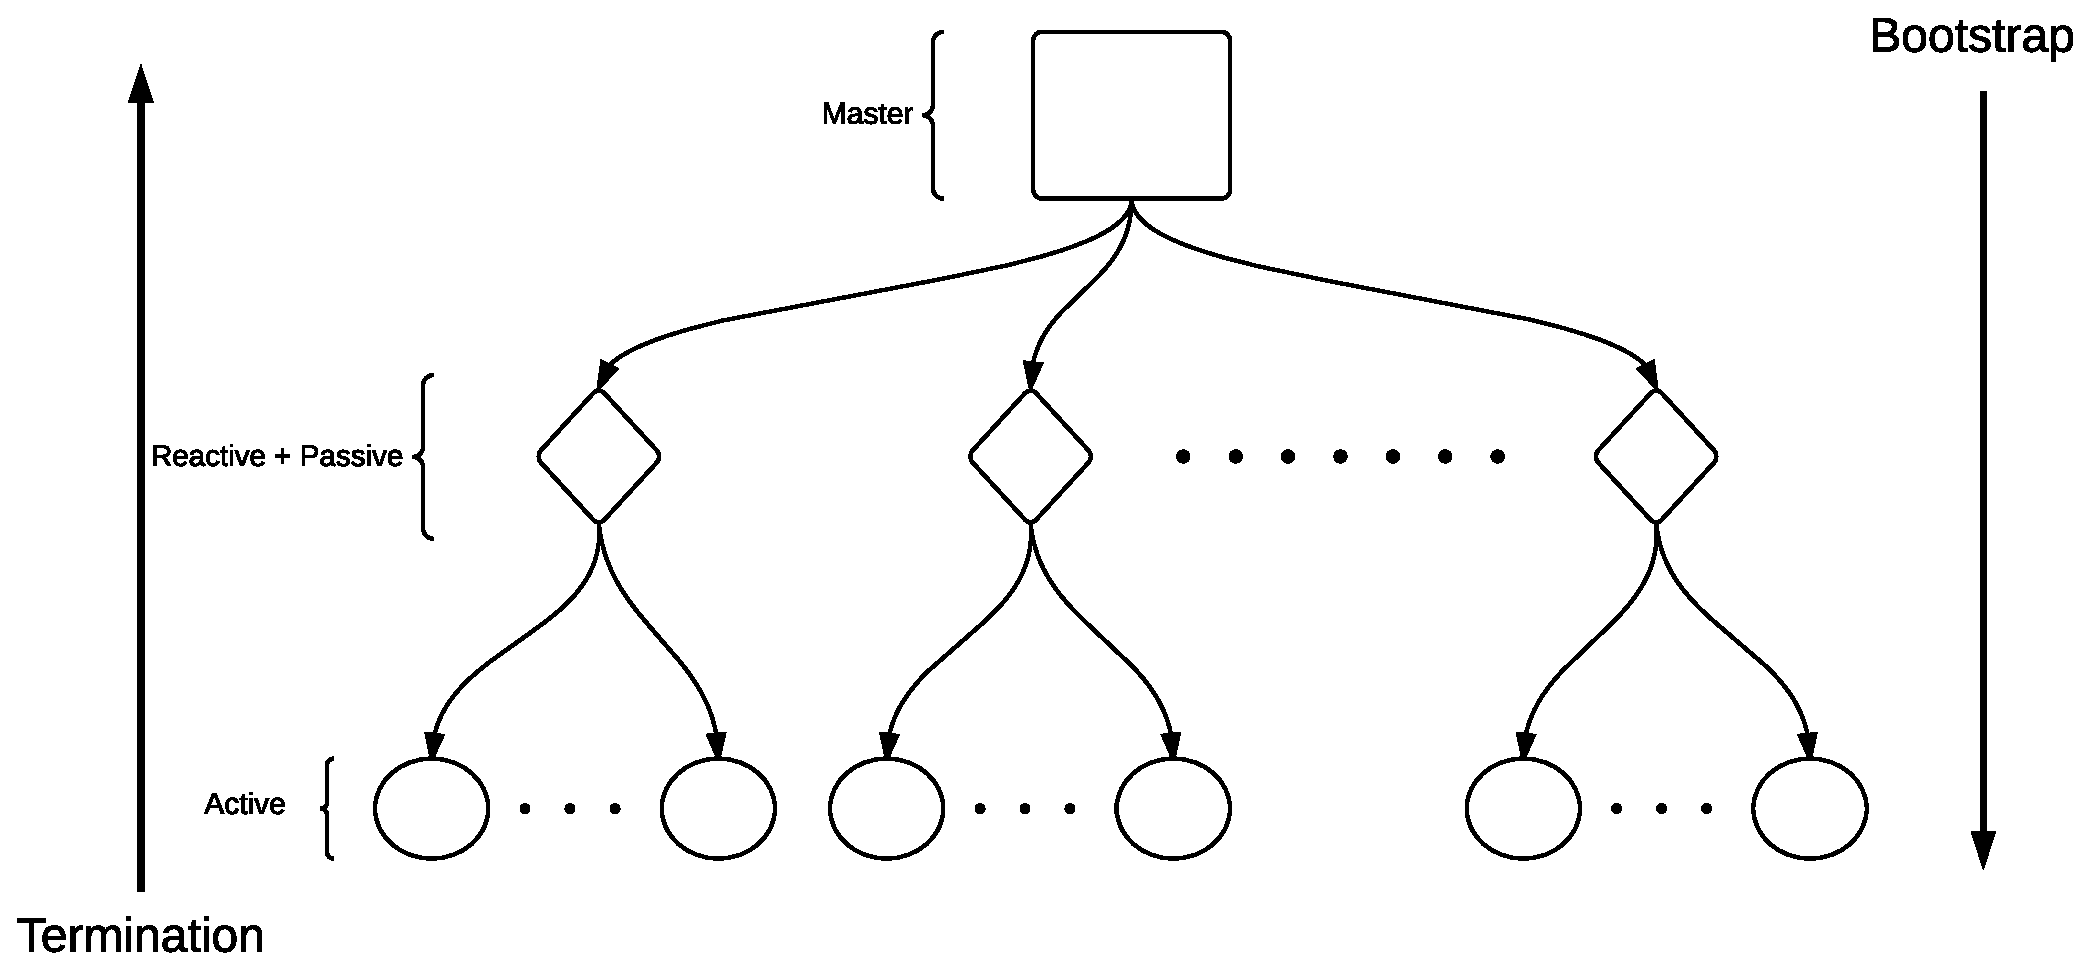
\includegraphics[width=\columnwidth]{images/solution/app_proc_tree.eps}
  \caption{Application process tree}
  \label{fig:app-proc-tree}
\end{figure}

At the end of the bootstrap, the \textit{Init} process has to notify the
middleware layer of the successful completion and the middleware has forwarded
the start message to the application. A crash of the
\textit{Init} process, occurring before the end of the bootstrap,
is signaled to the middleware layer, by the expiration of a timeout from the
middleware side.
Note that this model works also for a bootstrap which is executed starting
from a snapshot of the system, with the only difference consisting in divergent
values of the configuration file. Indeed, we have to use a set of
configurations, which is going to be different for each city.